\documentclass{standalone}
\usepackage{tikz}
\usetikzlibrary{patterns, positioning}
\usepackage[sfdefault]{ClearSans} %% option 'sfdefault' activates Clear Sans as the default text font
\usepackage[T1]{fontenc}

\begin{document}
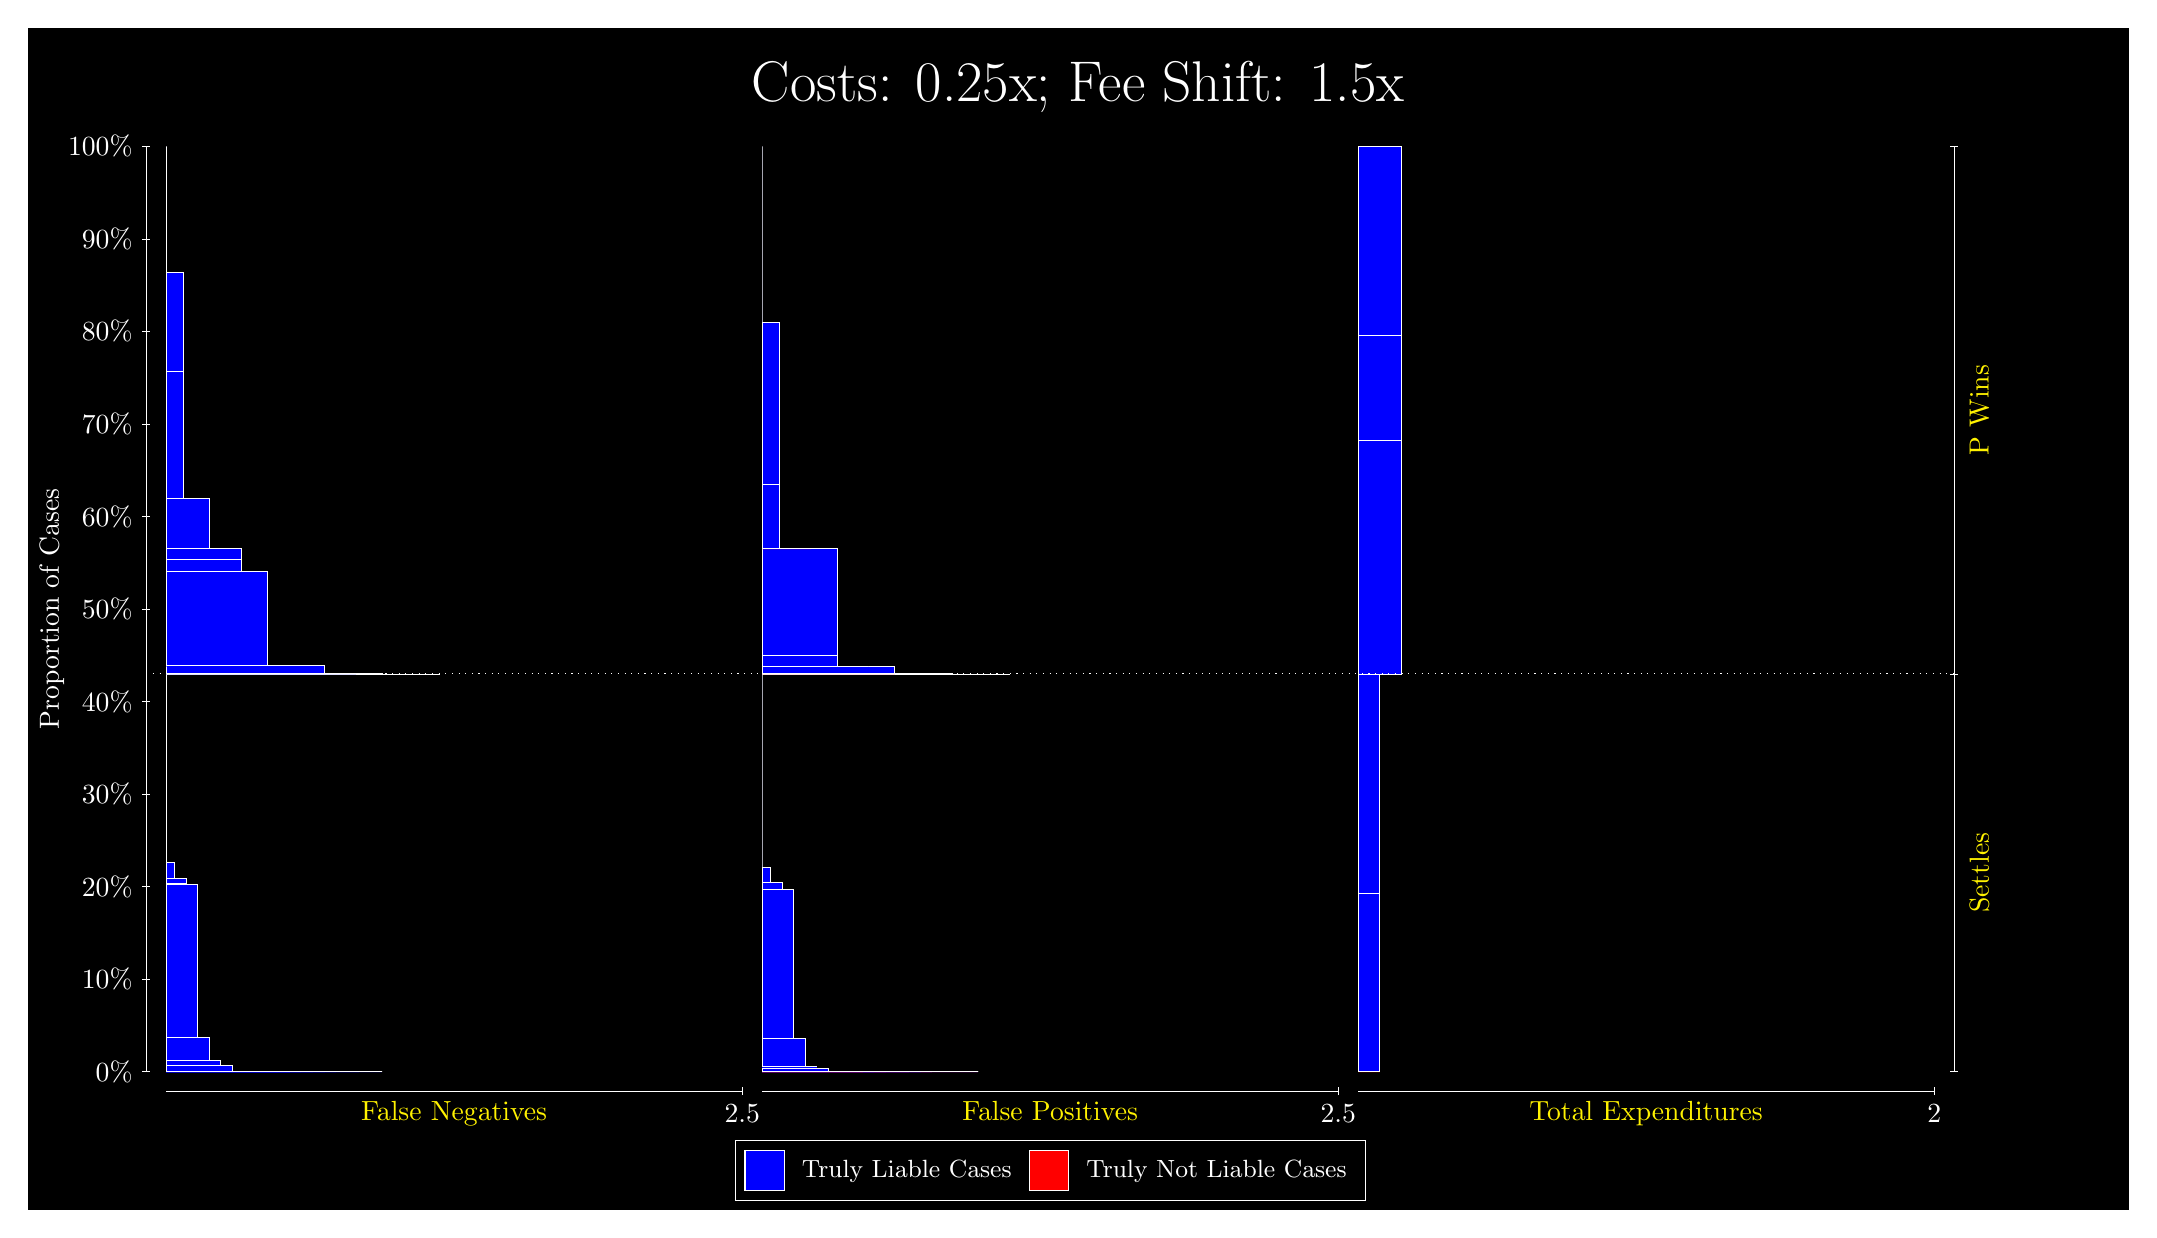
\begin{tikzpicture}
\draw[fill=black] (0,0) rectangle (26.667,15);
\draw[text=white] (0,13.5) rectangle (26.667,15) node[midway] {\huge Costs: 0.25x; Fee Shift: 1.5x};
\draw[white, very thin] (1.5,1.75) -- (1.5,13.5);
\node[rotate=90, text=white, anchor=center] at (0.3, 7.625) {Proportion of Cases};
\draw[white, very thin] (1.45,1.75) -- (1.55,1.75);
\node[text=white, anchor=east] at (1.45, 1.75) {0\%};
\draw[white, very thin] (1.45,2.925) -- (1.55,2.925);
\node[text=white, anchor=east] at (1.45, 2.925) {10\%};
\draw[white, very thin] (1.45,4.1) -- (1.55,4.1);
\node[text=white, anchor=east] at (1.45, 4.1) {20\%};
\draw[white, very thin] (1.45,5.275) -- (1.55,5.275);
\node[text=white, anchor=east] at (1.45, 5.275) {30\%};
\draw[white, very thin] (1.45,6.45) -- (1.55,6.45);
\node[text=white, anchor=east] at (1.45, 6.45) {40\%};
\draw[white, very thin] (1.45,7.625) -- (1.55,7.625);
\node[text=white, anchor=east] at (1.45, 7.625) {50\%};
\draw[white, very thin] (1.45,8.8) -- (1.55,8.8);
\node[text=white, anchor=east] at (1.45, 8.8) {60\%};
\draw[white, very thin] (1.45,9.975) -- (1.55,9.975);
\node[text=white, anchor=east] at (1.45, 9.975) {70\%};
\draw[white, very thin] (1.45,11.15) -- (1.55,11.15);
\node[text=white, anchor=east] at (1.45, 11.15) {80\%};
\draw[white, very thin] (1.45,12.325) -- (1.55,12.325);
\node[text=white, anchor=east] at (1.45, 12.325) {90\%};
\draw[white, very thin] (1.45,13.5) -- (1.55,13.5);
\node[text=white, anchor=east] at (1.45, 13.5) {100\%};

\draw[white, very thin] (24.457,1.75) -- (24.457,13.5);
\draw[white, very thin] (24.407,1.75) -- (24.507,1.75);
\node[anchor=west] at (24.407, 1.75) {};
\draw[white, very thin] (24.407,6.8004) -- (24.507,6.8004);
\node[anchor=west] at (24.407, 6.8004) {};
\draw[white, very thin] (24.407,13.5) -- (24.507,13.5);
\node[anchor=west] at (24.407, 13.5) {};

\draw[white, very thin, fill=blue] (1.75,1.75) rectangle (4.4946,1.75);
\draw[white, very thin, fill=blue] (1.75,1.75) rectangle (4.2018,1.75);
\draw[white, very thin, fill=blue] (1.75,1.75) rectangle (3.9091,1.75);
\draw[white, very thin, fill=blue] (1.75,1.75) rectangle (3.7627,1.75);
\draw[white, very thin, fill=blue] (1.75,1.75) rectangle (3.6163,1.75);
\draw[white, very thin, fill=blue] (1.75,1.75) rectangle (3.4699,1.75);
\draw[white, very thin, fill=blue] (1.75,1.75) rectangle (3.3236,1.7502);
\draw[white, very thin, fill=blue] (1.75,1.7502) rectangle (3.1772,1.7503);
\draw[white, very thin, fill=blue] (1.75,1.7503) rectangle (3.0308,1.7508);
\draw[white, very thin, fill=blue] (1.75,1.7508) rectangle (2.8844,1.7514);
\draw[white, very thin, fill=blue] (1.75,1.7514) rectangle (2.738,1.7541);
\draw[white, very thin, fill=blue] (1.75,1.7541) rectangle (2.5917,1.8312);
\draw[white, very thin, fill=blue] (1.75,1.8312) rectangle (2.4453,1.8904);
\draw[white, very thin, fill=blue] (1.75,1.8904) rectangle (2.2989,2.1892);
\draw[white, very thin, fill=blue] (1.75,2.1892) rectangle (2.1525,4.1234);
\draw[white, very thin, fill=blue] (1.75,4.1234) rectangle (2.0062,4.1405);
\draw[white, very thin, fill=blue] (1.75,4.1405) rectangle (2.0062,4.2013);
\draw[white, very thin, fill=blue] (1.75,4.2013) rectangle (1.8598,4.4027);
\draw[white, very thin, fill=red] (1.75,4.4027) rectangle (1.75,4.4027);
\draw[white, very thin, fill=blue] (1.75,4.4027) rectangle (1.75,6.8004);
\draw[white, very thin, fill=blue] (1.75,6.8004) rectangle (5.2265,6.8004);
\draw[white, very thin, fill=blue] (1.75,6.8004) rectangle (4.4946,6.8015);
\draw[white, very thin, fill=blue] (1.75,6.8015) rectangle (4.1652,6.8015);
\draw[white, very thin, fill=blue] (1.75,6.8015) rectangle (3.7627,6.9039);
\draw[white, very thin, fill=blue] (1.75,6.9039) rectangle (3.4333,6.9041);
\draw[white, very thin, fill=blue] (1.75,6.9041) rectangle (3.0308,8.1067);
\draw[white, very thin, fill=blue] (1.75,8.1067) rectangle (2.7015,8.2605);
\draw[white, very thin, fill=blue] (1.75,8.2605) rectangle (2.7015,8.3967);
\draw[white, very thin, fill=blue] (1.75,8.3967) rectangle (2.2989,9.0292);
\draw[white, very thin, fill=blue] (1.75,9.0292) rectangle (1.9696,10.648);
\draw[white, very thin, fill=blue] (1.75,10.648) rectangle (1.9696,11.905);
\draw[white, very thin, fill=red] (1.75,11.905) rectangle (1.75,11.905);
\draw[white, very thin, fill=blue] (1.75,11.905) rectangle (1.75,13.5);
\draw[white, very thin, fill=red] (9.3189,1.75) rectangle (12.063,1.75);
\draw[white, very thin, fill=blue] (9.3189,1.75) rectangle (12.063,1.75);
\draw[white, very thin, fill=red] (9.3189,1.75) rectangle (11.478,1.75);
\draw[white, very thin, fill=blue] (9.3189,1.75) rectangle (11.478,1.75);
\draw[white, very thin, fill=blue] (9.3189,1.75) rectangle (11.332,1.75);
\draw[white, very thin, fill=red] (9.3189,1.75) rectangle (11.185,1.75);
\draw[white, very thin, fill=blue] (9.3189,1.75) rectangle (11.185,1.75);
\draw[white, very thin, fill=red] (9.3189,1.75) rectangle (10.892,1.75);
\draw[white, very thin, fill=blue] (9.3189,1.75) rectangle (10.892,1.7501);
\draw[white, very thin, fill=blue] (9.3189,1.7501) rectangle (10.746,1.7501);
\draw[white, very thin, fill=red] (9.3189,1.7501) rectangle (10.6,1.7501);
\draw[white, very thin, fill=blue] (9.3189,1.7501) rectangle (10.6,1.7522);
\draw[white, very thin, fill=blue] (9.3189,1.7522) rectangle (10.453,1.7522);
\draw[white, very thin, fill=red] (9.3189,1.7522) rectangle (10.307,1.7522);
\draw[white, very thin, fill=blue] (9.3189,1.7522) rectangle (10.307,1.754);
\draw[white, very thin, fill=blue] (9.3189,1.754) rectangle (10.161,1.7907);
\draw[white, very thin, fill=red] (9.3189,1.7907) rectangle (10.014,1.7907);
\draw[white, very thin, fill=blue] (9.3189,1.7907) rectangle (10.014,1.8112);
\draw[white, very thin, fill=blue] (9.3189,1.8112) rectangle (10.014,1.8122);
\draw[white, very thin, fill=blue] (9.3189,1.8122) rectangle (9.8678,2.178);
\draw[white, very thin, fill=red] (9.3189,2.178) rectangle (9.7214,2.178);
\draw[white, very thin, fill=blue] (9.3189,2.178) rectangle (9.7214,4.0639);
\draw[white, very thin, fill=blue] (9.3189,4.0639) rectangle (9.7214,4.064);
\draw[white, very thin, fill=blue] (9.3189,4.064) rectangle (9.575,4.1477);
\draw[white, very thin, fill=blue] (9.3189,4.1477) rectangle (9.4287,4.3491);
\draw[white, very thin, fill=blue] (9.3189,4.3491) rectangle (9.3189,6.8004);
\draw[white, very thin, fill=red] (9.3189,6.8004) rectangle (12.466,6.8004);
\draw[white, very thin, fill=blue] (9.3189,6.8004) rectangle (12.466,6.8004);
\draw[white, very thin, fill=red] (9.3189,6.8004) rectangle (11.734,6.8004);
\draw[white, very thin, fill=blue] (9.3189,6.8004) rectangle (11.734,6.8015);
\draw[white, very thin, fill=red] (9.3189,6.8015) rectangle (11.002,6.8015);
\draw[white, very thin, fill=blue] (9.3189,6.8015) rectangle (11.002,6.903);
\draw[white, very thin, fill=red] (9.3189,6.903) rectangle (10.673,6.903);
\draw[white, very thin, fill=blue] (9.3189,6.903) rectangle (10.673,6.903);
\draw[white, very thin, fill=red] (9.3189,6.903) rectangle (10.27,6.903);
\draw[white, very thin, fill=blue] (9.3189,6.903) rectangle (10.27,7.0377);
\draw[white, very thin, fill=blue] (9.3189,7.0377) rectangle (10.27,8.3923);
\draw[white, very thin, fill=red] (9.3189,8.3923) rectangle (9.941,8.3923);
\draw[white, very thin, fill=blue] (9.3189,8.3923) rectangle (9.941,8.3952);
\draw[white, very thin, fill=blue] (9.3189,8.3952) rectangle (9.5384,9.2043);
\draw[white, very thin, fill=blue] (9.3189,9.2043) rectangle (9.5384,11.271);
\draw[white, very thin, fill=red] (9.3189,11.271) rectangle (9.3189,11.271);
\draw[white, very thin, fill=blue] (9.3189,11.271) rectangle (9.3189,13.5);
\draw[white, very thin, fill=red] (16.888,1.75) rectangle (17.162,1.75);
\draw[white, very thin, fill=blue] (16.888,1.75) rectangle (17.162,4.018);
\draw[white, very thin, fill=red] (16.888,4.018) rectangle (17.162,4.018);
\draw[white, very thin, fill=blue] (16.888,4.018) rectangle (17.162,6.8004);
\draw[white, very thin, fill=red] (16.888,6.8004) rectangle (17.437,6.8004);
\draw[white, very thin, fill=blue] (16.888,6.8004) rectangle (17.437,9.7671);
\draw[white, very thin, fill=red] (16.888,9.7671) rectangle (17.437,9.7671);
\draw[white, very thin, fill=blue] (16.888,9.7671) rectangle (17.437,11.098);
\draw[white, very thin, fill=red] (16.888,11.098) rectangle (17.437,11.098);
\draw[white, very thin, fill=blue] (16.888,11.098) rectangle (17.437,13.5);
\draw[white, dotted] (1.5,6.8004) -- (24.457,6.8004);
\draw[white, very thin] (1.75,1.5) -- (9.0689,1.5);
\node[text=yellow, anchor=north] at (5.4094, 1.5) {False Negatives};
\draw[white, very thin] (9.0689,1.45) -- (9.0689,1.55);
\node[text=white, anchor=north] at (9.0689, 1.45) {2.5};

\draw[white, very thin] (9.3189,1.5) -- (16.638,1.5);
\node[text=yellow, anchor=north] at (12.978, 1.5) {False Positives};
\draw[white, very thin] (16.638,1.45) -- (16.638,1.55);
\node[text=white, anchor=north] at (16.638, 1.45) {2.5};

\draw[white, very thin] (16.888,1.5) -- (24.207,1.5);
\node[text=yellow, anchor=north] at (20.547, 1.5) {Total Expenditures};
\draw[white, very thin] (24.207,1.45) -- (24.207,1.55);
\node[text=white, anchor=north] at (24.207, 1.45) {2};

\node[text=yellow, centered, rotate=90] at (24.777, 4.2752) {Settles};
\node[text=yellow, centered, rotate=90] at (24.777, 10.15) {P Wins};

\draw (12.978300999999998,1.5) node[draw=none] (baseCoordinate) {};
\begin{scope}[align=center]
        \matrix[scale=0.5, draw=white, below=0.5cm of baseCoordinate, nodes={draw}, column sep=0.1cm]{
            \node[rectangle, draw, minimum width=0.5cm, minimum height=0.5cm, fill=blue] {}; &
            \node[draw=none, font=\small, text=white] (B) {Truly Liable Cases}; &
            \node[rectangle, draw, minimum width=0.5cm, minimum height=0.5cm, fill=red] {}; &
            \node[draw=none, font=\small, text=white] (B) {Truly Not Liable Cases}; \\
            };
\end{scope}

\end{tikzpicture}
\end{document}